\documentclass[10pt,a4paper]{article}
\usepackage[margin=2.2cm]{geometry}
\usepackage{fontspec}
\usepackage{kotex}
\setmainfont{Apple SD Gothic Neo}
\setsansfont{Apple SD Gothic Neo}
\usepackage{amsmath,amssymb}
\usepackage{graphicx}
\usepackage{caption}
\usepackage[dvipsnames]{xcolor}
\usepackage[colorlinks=true,linkcolor=MidnightBlue,citecolor=MidnightBlue,
            urlcolor=MidnightBlue]{hyperref}
\usepackage{titlesec}
\titleformat{\section}{\large\bfseries}{\thesection}{0.6em}{}
\captionsetup{font=small,labelfont=bf}
\setlength{\parskip}{0.35em}
\setlength{\parindent}{0pt}
\usepackage{mdframed}
\newmdenv[linewidth=0.4pt,linecolor=gray!60,backgroundcolor=gray!5,
          innertopmargin=6pt,innerbottommargin=6pt,skipabove=8pt,skipbelow=8pt]{claimbox}
\newcommand{\claim}[2]{\begin{claimbox}\textbf{주장.} #1\par\smallskip
  \textcolor{gray!70}{\textbf{반증 조건.} #2}\end{claimbox}}

\title{\bfseries 조건부 자로도 기저는 없다\\[2pt]
\large $819$ 문패 종결 --- 그리고 아이돌이 이웃을 얻었다}
\author{월드모델 실험실 · 노트 $841$}
\date{2026-08-08}
\begin{document}\maketitle

\section{한 줄}

$819$ 의 등록 미결(치환 중요도는 상관 축의 몫을 가른다)을 이행했다: 학습 구간
$|r| \geq 0.5$ 로 병합한 \textbf{상관 무리 $32$개} 단위의 조건부 치환,
$12$도메인 $66$쌍. \textbf{널 초과 $15/66 = 23\% \leq 35\%$ --- 확정.}
``합동은 공유 기저를 안 쓴다''($819$)는 상관-몫 인공물이 아니었고, 문패가
종결됐다(예측 $60\%$ 적중 · seed$0$ 판 $0.4738$ 재현 · 그룹 천장
$0.75{\sim}1.00$ 으로 축 단위보다 안정).

\begin{figure}[t]\centering
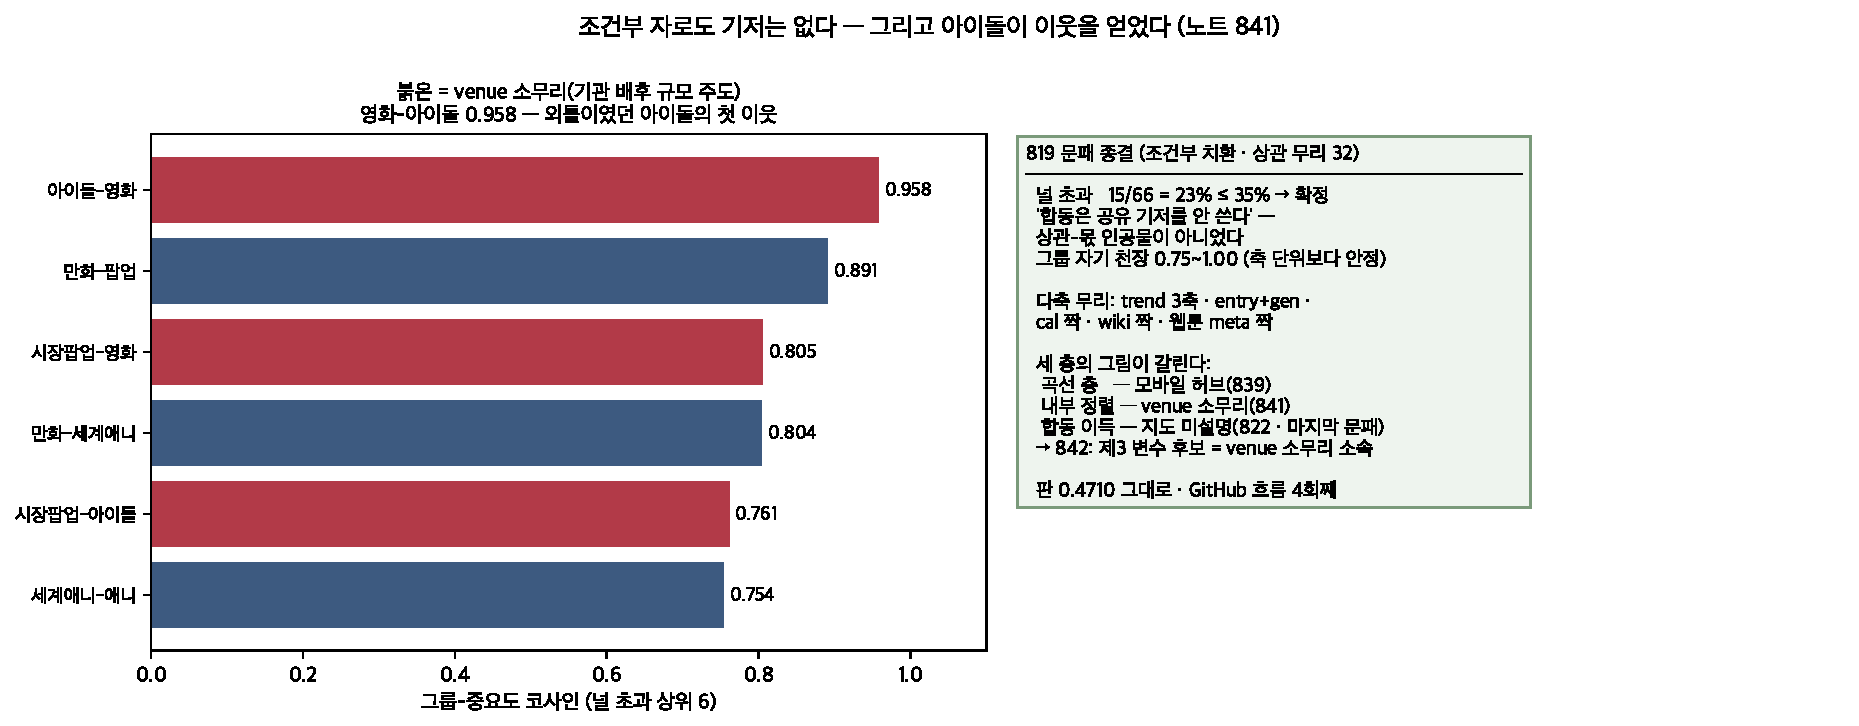
\includegraphics[width=0.97\textwidth]{figs/venue.pdf}
\caption{왼쪽: 널 초과 상위 쌍 --- 붉은 것이 venue 소무리. 오른쪽: 결산.}
\end{figure}

\section{venue 소무리 --- 세 층의 그림이 갈린다}

\claim{\textbf{영화의 모델-내부 최근접은 아이돌이다(cos $0.958$)} --- 시장팝업-영화
$0.805$ · 시장팝업-아이돌 $0.761$ 과 함께 \textbf{venue\_prominence(기관 배후
규모 --- 소속사 · 배급사 · 기사화)가 주도하는 소무리}가 드러났다. 부 예측
(`모바일 아닐 것' $55\%$) 적중: \textbf{곡선 층(모바일 허브 · $839$)과
모델-내부 정렬(venue 소무리)은 다른 구조}다. $819$ 에서 외톨이(`방향이
다르다' 교차 최하위)였던 아이돌이 영화 합류로 처음 이웃을 얻었다 ---
TabPFN 보조 헤드 서사($803{\sim}$)의 새 조명이다.}
{마지막 문패 $822$(합동 이득 지도의 제$3$ 변수)의 유력 후보가 생겼다:
\textbf{venue 소무리 소속 여부}. $842$ 에서 잰다. GitHub 흐름 $4$회째 완주
(이슈 \#$8 \to$ PR \#$9$). 판 $\rho$ $0.4710$ 그대로.}

\end{document}
